\documentclass[10pt,a4paper]{article} \usepackage[utf8]{inputenc}
\usepackage[obeyDraft]{todonotes}
\usepackage{hyperref}
\usepackage{amssymb}
\usepackage{multirow}
\usepackage{footnote}
\usepackage{parskip}
\usepackage{xspace}
\usepackage[T1]{fontenc}
\makesavenoteenv{tabular}
\makesavenoteenv{table}

%---------------------------------------------------------------------------------------------------
\title{JACUSA2 manual}
\author{Michael Piechotta \\ michael.piechotta@gmail.com}
\date{9th, October, 2019} 
%---------------------------------------------------------------------------------------------------
\begin{document}
\newcommand{\call}[1]{\textit{call-#1}\xspace}
\newcommand{\pileup}{\textit{pileup}\xspace}
\newcommand{\rtarrest}{\textit{rt-arrest}\xspace}
\newcommand{\lrtarrest}{\textit{lrt-arrest}\xspace}
%---------------------------------------------------------------------------------------------------
\maketitle
\tableofcontents
\listoftodos
%---------------------------------------------------------------------------------------------------
\newpage
%---------------------------------------------------------------------------------------------------
\section{Introduction}
JAVA framework for accurate Variant assessment (JACUSA2) is a one-stop solution to detect single
nucleotide variants (SNVs) and reverse transcriptase induced arrest events in Next-generation
sequencing (NGS) data.

\url{https://github.com/dieterich-lab/JACUSA2/}{JACUSA2} is a direct successor of
\url{https://github.com/dieterich-lab/JACUSA/}{JACUSA1} --- JACUSA1 is hereby deprecated and won't
be continued. All methods from JACUSA1 (\call{1}, \call{2}, and \pileup) are available in JACUSA2.

The new release offers great performance enhancements (~3 faster) for existing methods
and adds new methods (\rtarrest and \lrtarrest) to identify read arrest events by means of comparing 
read through and read arrest counts. \lrtarrest is a combination of \call{2} and \rtarrest that 
allows to identify such linked variant and arrest events.
\begin{figure}[ht]
  \centering
  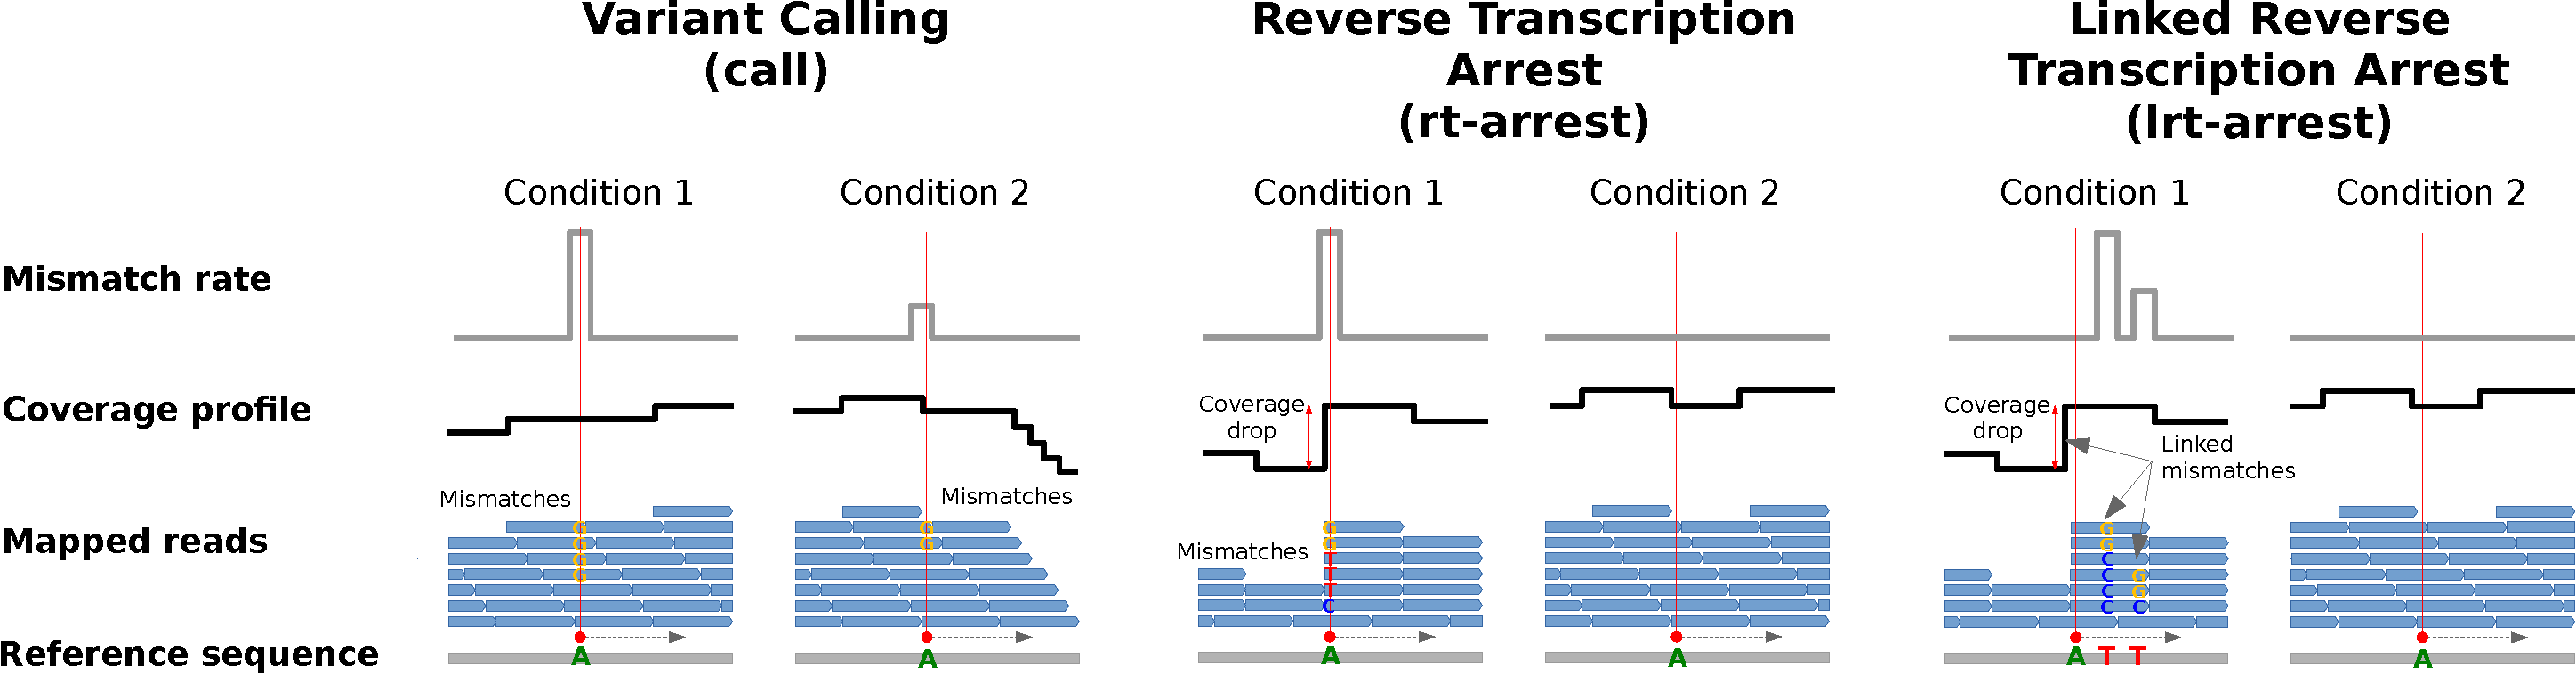
\includegraphics[width=\textwidth]{figures/jacusa_methods_cropped}
  \caption{Schematic summary of JACUSA2 methods and underlying characteristics of data.}
  \label{fig:methods}
\end{figure}
Robust identification of variants has proven to be a daunting task due to artefacts specific for
NGS-data and employed mapping strategies. We implement various artefact/feature filters that reduce
the number of false positives (see section \ref{sec:artefact_filter}). A new feature filter has been
added to JACUSA2 to filter candidate variants or arrest events by providing a file with sites to be
excluded.
Some artefact filters have been moved from JACUSA1 to the R helper package called JACUSA\textbf{2}helper\footnote{Check
\url{https://github.com/dieterich-lab/JACUSA2helper}}.

Another new feature, are optional data that can be added to the output of some methods.
Such optional data are INDEL counts and associated differential statistics and read substitution
information. A user defined base substitution can be used to partition reads into two sets
\todo[author=cd]{what is a typical experiment for this?}.

JACUSA2 employs a window-based approach to traverse BAM \cite{HengLi2009} files, featuring highly
parallel processing and utilizing the htsjdk\footnote{Check \url{https://github.com/samtools/htsjdk}} 
framework.
%---------------------------------------------------------------------------------------------------
\subsection{Variant calling}
\begin{figure}[ht]
  \centering
  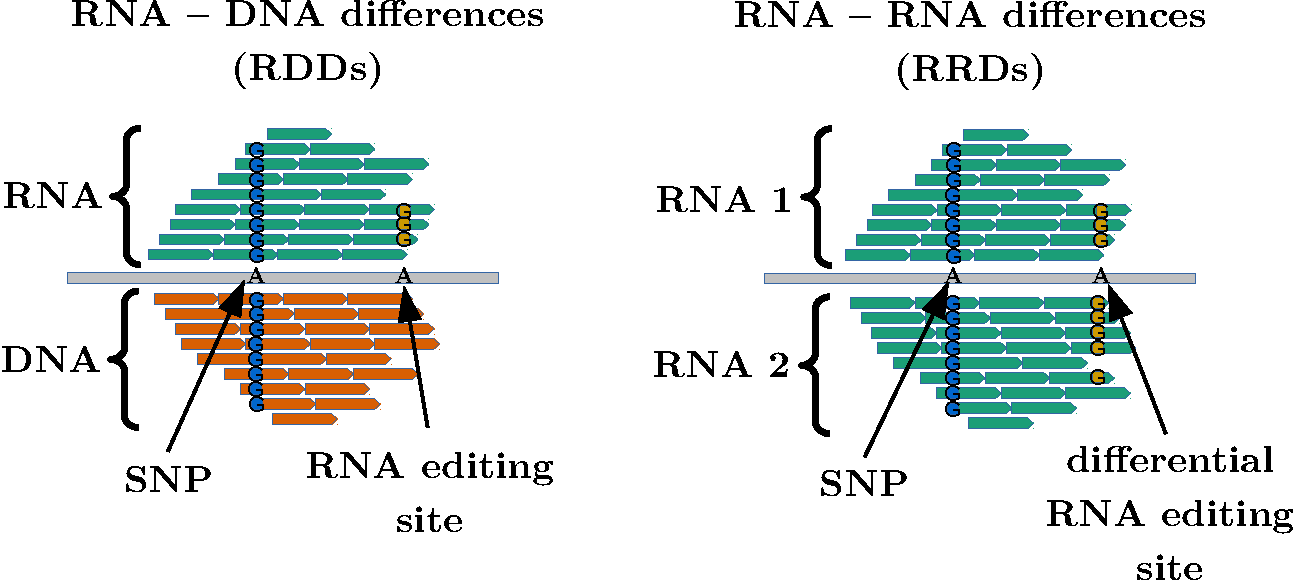
\includegraphics[width=.6\textwidth]{figures/dres_cropped}
  \caption{Identification of RNA-editing sites in JACUSA2}
  \label{fig:dres}
\end{figure}
JACUSA2 has been extensively evaluated and optimized to identify RNA editing sites in RNA-DNA and
RNA-RNA sequencing samples (see Figure \ref{fig:dres}). Checkout the original publication and the
supplementary material of JACUSA1 \cite{Piechotta2017} if you are interested in details regarding
the test-statistic.
%---------------------------------------------------------------------------------------------------
\subsection{Reverse transcriptase arrest events}
\begin{figure}[ht]
  \centering
  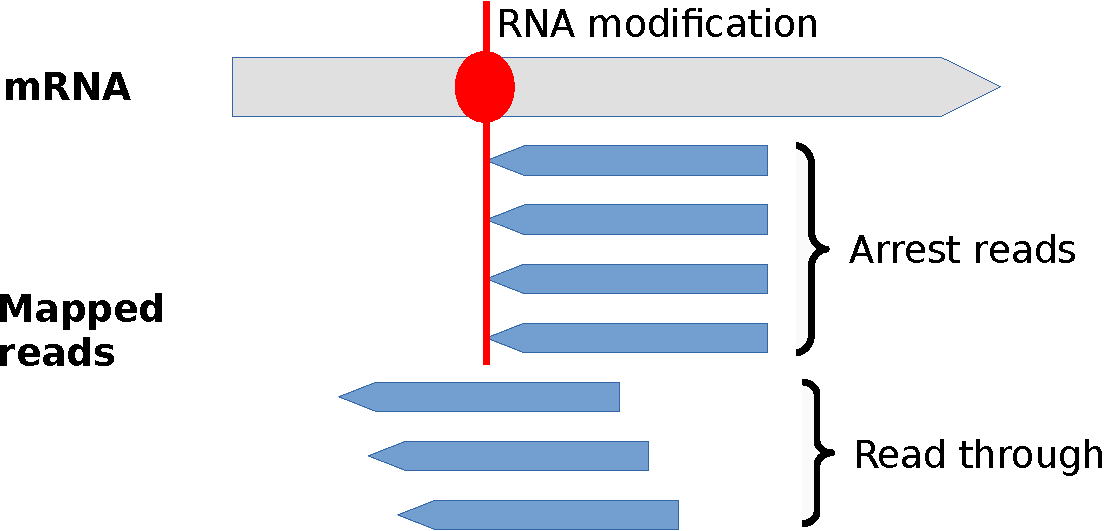
\includegraphics[width=.6\textwidth]{figures/arrest_events_cropped}
  \caption{Schematic depiction of arrest events that have been induced by modifications that
  influence reverse transcription during library preparation}
  \label{fig:arrest_event}
\end{figure}
Reverse transcriptase arrest events can be induced during library preparation (see Figure
\ref{fig:arrest_event}).
They are identified by reads that exhibit shorter than expected read length due to premature
termination during first strand synthesis. For each site, a vector of read through and read arrest
counts is constructed and modelled with a Beta-Binomial distribution. We estimate the parameters of
the distribution with the method presented by Minka\footnote{Check 
\url{https://tminka.github.io/papers/dirichlet/minka-dirichlet.pdf}}.
% --------------------------------------------------------------------------------------------------
\section{Download}
The latest version of JACUSA2 can be obtained from
\url{https://github.com/dieterich-lab/JACUSA2}.

Go to \url{https://github.com/dieterich-lab/JACUSA2/releases} and pick the lastest
release.
% --------------------------------------------------------------------------------------------------
\subsection{Installation and requirements}
JACUSA2 does not need any configuration but needs a correctly configured Java environment.
We developed and tested JACUSA2 with Java v1.8. If you encounter any Java related problems please
consider to change to Java v1.8.
% --------------------------------------------------------------------------------------------------
\subsection{Migrating from JACUSA1 to JACUSA2}\label{sec:migration}
There are several important changes to the command line interface:
\begin{itemize}
  \item ONLY single dash ``-'' options, e.g.: ``-c 10'' are supported. ALL two dash options
  ``--option [\ldots]'' from JACUSA1 have been removed.
  \item Use ``\textbf{-}filterNH'' and ``\textbf{-}filterNM'' instead of ``--filterNH'' and
  ``--filterNM''.
  \item CLI option to provide library type has changed: JACUSA1: ``-P Lib1,Lib2'' $\rightarrow$
  JACUSA2: ``-P1 Lib1 -P2 Lib2''.
  \item Artefact/feature filter has now named options, e.g.: JACUSA1: ``-a H:1'' $\rightarrow$
  JACUSA2: ``-a H:\textbf{condition=1}''. Check Section \ref{sec:cli_artefact_filter} for details.
  \item Test-Statistic options ``-u <STAT>`` have named options.
\end{itemize}
A \#\#'' prefixed header line has been added to the default output format of JACUSA2. The header
line contains version and command line info.
There is also a new version of JACUSA\textbf{2}helper\footnote{Check 
\url{https://github.com/dieterich-lab/JACUSA2helper/}} to support downstream
analysis of JACUSA2 output. JACUSAhelper has been declared deprecated and won't be maintained
anymore.
%TODO 4==5 counts for filters 0-index vs. index
%different homopolymer filter, filtering adjacent
% --------------------------------------------------------------------------------------------------
\subsection{\textit{In silico} and example data}
\subsubsection{Variant calling}
You can choose between different \textit{in silico} setups to detect variants. 

The gDNA vs. cDNA represents the typical data setup that is encountered in detection of RNA editing
sites via comparing genomic and transcriptomic sequencing reads. In this setup, variants have been
only imputed to the cDNA BAM file.

The cDNA vs. cDNA data setup can be interpreted as representing allele specific expression of single
variants or differential RNA editing. In this setup, variants with pairwise different base
frequencies have been imputed into both cDNA BAM files. Additionally, to make the identification of
variants more challenging, SNPs with pairwise similar base frequencies have been included to both
BAM files. SNPs should not be identified as true positive sites.

gDNA data has been simulated with art\footnote{Check
\url{http://www.niehs.nih.gov/research/resources/software/biostatistics/art}} and cDNA reads
have been simulated with flux simulator\footnote{Check \url{http://sammeth.net/confluence/display/SIM/Home}}.
Read simulations have been restricted to the corresponding first chromosome of human. Simulated BAM
files have been processed and only reads with mapping quality $\ge 20$ have been retained. Check
Table \ref{tbl:call_data} for details about contents of available data.

\todo[author=mp]{Add readme to archives, check link}:
\newcommand{\callRDD}{gDNA vs. cDNA: \url{https://data.dieterichlab.org/s/gDNA_VS_cDNA}}
\newcommand{\callRRD}{cDNA vs. cDNA: \url{https://data.dieterichlab.org/s/cDNA_VS_cDNA}}
\begin{table}
  \centering
  \caption{Detailed description of available \textit{in silico} data for variant calling. Data has been simulated on human chromosome 1 using hg19.}
  \label{tbl:call_data}
  {\small
  \begin{tabular}{llp{.5\textwidth}}
    \textbf{Setup} & \textbf{File} & \textbf{Description} \\
    \hline
    \hline
    \multirow{3}{*}{gDNA vs. cDNA \footnote{\callRDD}} & gDNA.bam     & Simulated genomic DNA \\
                                                      & cDNA.bam     & Simulated RNA-Seq data \\
                                                      & variants.txt & Coordinates of imputed variants and their target 
                                                                          and sampled frequencies. \\
    \hline
    \multirow{4}{*}{gDNA vs. cDNA \footnote{\callRRD}} & cDNA\_1.bam  & Simulated RNA-Seq data for 1st condition. \\
                                                        & cDNA\_2.bam  & Simulated RNA-Seq data for 2nd condition. \\
                                                        & variants.txt & Coordinates of imputed variants and their target 
                                                                            and sampled frequencies. \\
                                                        & snps.txt     & Coordinates of imputed SNPs. In both BAM files 
                                                                            matching SNPs have the same target frequency but 
                                                                            different effective or sampled frequencies. The 
                                                                            shape parameter determines how much the sampled 
                                                                            frequency will deviate from the target frequency. 
                                                                            The suffixes: 1 and 2 correspond 
                                                                                to the respective BAM file.
  \end{tabular}}
  
\end{table}
% --------------------------------------------------------------------------------------------------
\subsubsection{Reverse transcriptase arrest events}
We have downloaded primary sequencing data from \cite{Zhou2018} and mapped them according to
\todo[author=christoph]{How did we do this?}.
From the resulting read sets, we retained only read uniquely mapping to 18S and 28S rRNAs with
mapping quality $\ge 20$.
\cite{Zhou2018} map RNA modification of pseudouridine ($\Psi$) by chemically modifying
pseudouridines with carbodiimide (+CMC) and detecting arrest events that are induced by reverse
transcription stops in high-throughput sequencing under 3 different conditions (HIVRT, SIIIMn, and
SIIIMg).

The archive \url{https://data.dieterichlab.org/s/arrest_events} consists of:
\begin{description}
  \item[*.bam, *.bam.bai] BAM files and BAM indicices for different 3 conditions HIVRT, SIIIRTMg,
  and SIIIRTMn each treated with CMC(+CMC) or mock-treated(-CMC) (6 BAM + 6 BAI files).
  \item[fournier\_db.txt] Parsed and coordinate adjusted list of known modifications for human 18S
  and 28S according to Fournier lab's 3D rRNA modification maps database \cite{PieknaPrzybylska2007}.
  \item[README.txt] Summary of referenced data and original data sources. Read for details.
\end{description}
%---------------------------------------------------------------------------------------------------
\section{Input/Output}
All JACUSA2 methods require sorted and indexed BAM\footnote{Check 
\url{https://samtools.github.io/hts-specs/SAMv1.pdf}} files.
BAM is a standardized file format for efficient storage of alignments.
Furthermore, JACUSA2 requires that the reference sequence is available either through the ``MD''-tag
\footnote{Check \url{https://samtools.github.io/hts-specs/SAMtags.pdf}} in BAM files or by providing 
the reference sequence in indexed FASTA format with the command line option ``-R <reference.fasta>''.
The ``MD'' field contains mismatch information that allows to perform variant calling without
providing the reference sequence.

Check the manuals of: SAMtools/BCFtools\footnote{Check \url{http://samtools.sourceforge.net/}} and/or
picard tools\footnote{\url{http://broadinstitute.github.io/picard/}} for how to use the respective tool to
convert your alignment files to valid JACUSA2 input BAM.
%---------------------------------------------------------------------------------------------------
\subsection{Processing BAM files}
In the following, commands for SAMtools\footnote{Check \url{http://www.htslib.org}} are presented.

To sort and index your raw BAM files, perform the following sequence of commands:
\begin{description}
  \item[SAM $\rightarrow BAM$] \begin{verbatim} samtools view -Sb mapping.sam > mapping.bam
  \end{verbatim} \item[sort BAM] \begin{verbatim} samtools sort mapping.bam mapping.sorted
  \end{verbatim} \item[index BAM] \begin{verbatim} samtools index mapping.sorted.bam \end{verbatim}
\end{description}

Check your BAM file for the ``MD''-tag if you want to provide reference sequence information via this 
tag. When your BAM files do not have the ``MD'' tag properly set, use SAMtools:
\begin{verbatim}
samtools calmd mapping.sorted.bam reference.fasta > mapping.sorted.MD.bam
\end{verbatim}
%---------------------------------------------------------------------------------------------------
\subsubsection{Remove duplicates for variant calling}
It is a recommended pre-processing step to remove duplicated reads when identifying variants -
\textbf{omit this step for \rtarrest and \lrtarrest}. Reads that are terminated prematurely during
library preparation will falsely be identified as PCR duplicates and removed from the final output.
This will dramatically degrade sensitivity for arrest event idetification.

Duplicated reads occur mostly due to PCR-artefacts. They are likely to harbour false variants and
most statistical test require independently sampled reads.
In the following, commands for picard tools are
presented:
\begin{verbatim} java -jar MarkDuplicates.jar \
  I=mapping.sorted.bam O=dedup_mapping.sorted.bam \
  M=duplication.info
\end{verbatim}
Most tools either remove duplicated reads from the final output or assign 1024 to the flag\footnote{
Check \url{https://broadinstitute.github.io/picard/explain-flags.html}} field of those reads. In the
later case, invoke JACUSA2 with the additional command line option ``-F 1024'' to filter reads that
have been marked as duplicated (See Section \ref{sec:filter_flag}).
%---------------------------------------------------------------------------------------------------
\subsubsection{Library type and strand information}
JACUSA2 supports stranded paired end (PE) and single ends (SE) reads. \textbf{Warning:} the CLI option
has changed (see Section \ref{sec:migration})!

With the command line parameter ``-P <LIBRARY-TYPE> '' or '' -P1 <LIBRARY-TYPE> -P2 <LIBRARY-TYPE>''
the user can choose from the following supported library types:
\begin{description} 
\item[RF-FIRSTSTRAND] STRANDED library - first strand sequenced,
\item[FR-SECONDSTRAND] STRANDED library - second strand sequenced, and
\item[UNSTRANDED] UNSTRANDED library.
\end{description}
The ``UNSTRANDED'' is not available for \rtarrest and \lrtarrest method because an arrest site can
not be unambiguously defined for this library type. Read base substitution option ``-B <BASE-SUB>''
requires a stranded library type in order to corretly identify base substitutions based on strand 
information.
%---------------------------------------------------------------------------------------------------
\subsection{BED-like search region}
Identification of interesting sites can be restricted to specific regions of the genome or transcriptome.
Provide a minimalistic BED-like file to limit the search to some region(s) or site(s). 
Complementary region(s) of the BAM files will not be considered.

In the following file, the search is confined to a 100nt region on contig 1
starting at position 1,000 and a single site on contig 2 at position 10,000:
\begin{table}
\centering
  \caption{Definiton of an exemplary BED-like search region}
  \label{tbl:search_region}
  \begin{tabular}{lll}
    \textbf{contig} & \textbf{start} & \textbf{end} \\
    \hline
    1 & 1000 & 1100 \\
    2 & 10000 & 10000 \\
    \multicolumn{3}{c}{}
  \end{tabular}
\end{table}
Many individual sites may impair running performance of JACUSA2.
Try to merge nearby sites to create contiguous regions and extract specific sites from 
JACUSA2 output with bedtools\footnote{\url{http://bedtools.readthedocs.org/en/latest/}} ``intersect'':
\begin{description}
\item[merge sites] \begin{verbatim} 
bedtools merge -d 500 singular_sites.bed > \
  contigous_regions.bed
\end{verbatim}
\item[run JACUSA2] \begin{verbatim} 
java -jar JACUSA2.jar call-2 -b contigous_regions.bed \ 
  -r JACUSA2.out mapping_1.sorted.bam mapping_2.sorted.bam
\end{verbatim}
\item[extract sites] \begin{verbatim}
bedtools intersect -wa -a JACUSA2.out -b singular_sites.bed
\end{verbatim}
\end{description}
%---------------------------------------------------------------------------------------------------
\subsection{General output format}
JACUSA2 writes its output to a user specified file. When using multiple threads, JACUSA2 will
create a temporary file for each allocated thread in the temp directory that is provided by the 
JAVA Virtual Machine. Check the manual of your JAVA Virtual machine on how to change the temp directory. 

Chosen command line parameters and current genomic position are printed to the command prompt and
serve as a status guard. Furthermore, depending on the provided command line parameters, JACUSA2
will generate a file with sites that have been identified as potential artefacts when ``-s'' is
provided.

Output format of JACUSA2 is controlled by the ``-f <FORMAT>'' command line option. Support for output 
formats depends on the used method. Check Table \ref{tbl:method2format} for a summary of currently 
supported output formats.
\newcommand{\vcfspec}{Check \url{http://samtools.github.io/hts-specs/VCFv4.1.pdf}}
\begin{table}[ht]
  \centering
  \caption{Summary of available output formats for each method.}
  \label{tbl:method2format}
  \begin{tabular}{lcccc}
                                                 & \multicolumn{4}{c}{\textbf{Method}} \\
    \textbf{Output format}                       & \call{1,2} & \pileup & \rtarrest & \lrtarrest \\
    \hline
    JACUSA2 BED-like format                      & x        & x       & x         & x \\
    Variant Call Format (VCF\footnote{\vcfspec}) & x        & x       &           & \\
  \end{tabular}
\end{table}
The default output format is combination of
BED6\footnote{Check \url{http://genome.ucsc.edu/FAQ/FAQformat.html\#format1}} with
JACUSA2 methods specific columns and common info column: ``info'', ``filter\_info'', and
 ``ref\_base''.

A ``\#\#'' prefixed header that contain JACUSA2 runtime specific info such as version info and
command line options is added to the default output format. The actual number of columns depends on
the JACUSA2 method and the number of provided BAM files.

Check table \ref{tbl:general_output} for a general description of JACUSA2 output format and check
method or option specific adjustments in the following sections:
\begin{itemize}
  \item \rtarrest method \ref{sec:rt_arrest},
  \item \lrtarrest method \ref{sec:lrt_arrest},
  \item optional INDEL data fields \ref{sec:indel}, or
  \item base substitution based read stratification \ref{sec:read_base_stratification}.
\end{itemize}
\begin{table}[ht]
  \centering 
  \caption{General description of JACUSA2 default output format with exemplary \call{2}
  output --- ``N'' corresponds to the total number of columns. Check detailed explanation of columns
  under the table.}
  \label{tbl:general_output}
{\small
\begin{tabular}{l|cccccc|ccc|cc}
         & \multicolumn{6}{c|}{\textbf{BED6 columns}} & \multicolumn{3}{c}{\textbf{Method specific}} & \multicolumn{2}{c}{\textbf{Additional}} \\
Column:  & 1 & 2 & 3 & 4 & 5 & 6 & 7 & \ldots & N-2 & N-1 & N \\
\hline
Example: & 1 & 100 & 101 & call & $8.07$ & - & 0,0,0,10 & \ldots & 0,2,0,10 & * & * \\
         & \multicolumn{6}{c|}{\ldots} & \multicolumn{3}{c}{\ldots} & \multicolumn{2}{c}{\ldots} \\
\end{tabular}}
\end{table}
\begin{description}
  \item[(1, 2, 3) contig + start + end] 0-indexed coordinates $[start, end)$.
  \item[(4) name] String that depends on method. Currently has no use except to ensure BED6 compatibility.
  \item[(5) score] Score for this site. ``*'' if not available. Depends on actual method.
  \item[(6) strand] Possible values are: ``.'', ``+'', and ``-'' which correspond to ``unstranded'',
  ``positive strand'', and ``negative strand'', respectively. If strand is ``= ``.'', then columns
  with base call information will be showing base counts \textbf{according} to the strand --- inverted
  base count if on the ``negative strand''.
  \item[(7 --- N-3) method specific] The number of base columns depends on the JACUSA2 method and
  the number of BAM files --- check method specific explanation.
  \item[(N-2) info] Additional info for this site. Actual content depdents on method and command
  line parameters. Details about the parameter estimation of the underlying distribution can be shown,
  insertion/deletion counts, and additional method specific data. If nothing  provided, set to ``*''. 
  The ``info'' field is used to add optional site specific data without changing 
  the total number of columns.
  \item[(N-1) filter\_info] Relevant, if artefact/feature filter(s) $X$ have been provided with 
  ``-a X'' on the command line. The column will contain a comma-separated list of artefact/feature 
  filters that recognised this site. Will be ``*'' if empty.\\
  \item[(N) ref\_base] The reference base according to coordinats and (6) strand information --- 
  Inverted if on the ``negative strand''.
\end{description}
%---------------------------------------------------------------------------------------------------
\section{Artefact/feature filter}
False positive variant calls can be related to mapping artefacts and sequencing technology.
Short read mappers tend to produce incorrect alignments around INDEL positions that may be falsely identified as variant sites.
Other false variant calls originate from uneven base call error distributions along short reads.
We have implemented a panel of simple threshold based artefact filters. Beyond artefacts, we have added filters
that identify some features of a pileup or a read and can be used to mark those sites.

When a site is identified by an artefact or feature filter $X$, $X$ is added to the ``filter\_info'' column 
and optionally this site can be moved to an other output file when command line ``-s [FILTERED-OUTPUT]'' has been used.
This strategy presevers all sites and allows the user investigate the fraction of filtered vs. total calls. 
In the following, we will use artefact and feature filtered interchangeably and a site we will call a site removed 
by a feature filter albeit the site is marked by the ID of feature filter.

When identifying RDDs by comparing gDNA vs. cDNA, it is common practice to remove or mask sites that 
are homozygous in gDNA (feature filter H) and have more than three distinct base types (artefact filter M).

We have added the exclude site filter in JACUSA2 that allows to mark sites in the final output as 
overlapping with sites/regions that are contained in a file. The supported file type are: VCF, BED, or JACUSA2 output. 
Given a set of known SNPs, polymorphic sites can be directly marked and removed from the list of 
candidate RNA-editing sites are identified by JACUSA2 in gDNA vs. cDNA or cDNA vs. cDNA comparisons:
\begin{verbatim}
java -jar JACUSA2.jar -a E:file=snps.vcf:type:VCF -r JACUSA2.out cDNA-1.bam cDNA-2.bam
\end{verbatim}
For performance reasons, the input file is required to be sorted by coordinate --- \textbf{WARNING:} 
Sort order is not tested within JACUSA2.

Our filters (D,B,I,Y) monitor the distance d of a given candidate site to relevant read features such as start/end, 
INDEL positions, homopolymeric regions, and splice sites and remove the candidate site from further 
consideration if a proportion r of all reads falls below the given distance cutoff $\le d$.
\begin{figure}[h]
  \centering
  \caption{Summary of available artefact/feature filters for each method and examples.}
  \label{fig:method2artefact_filter}
  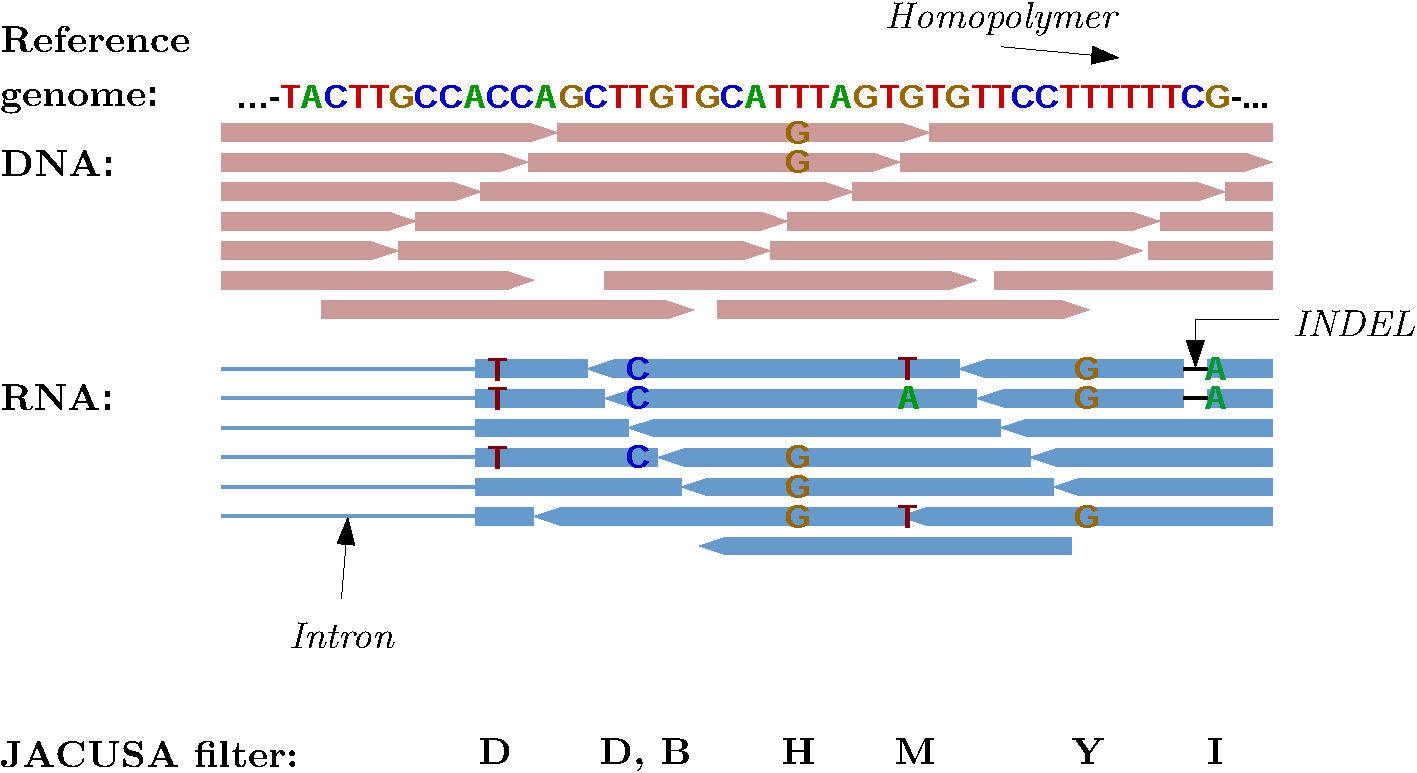
\includegraphics[width=\textwidth]{figures/jacusa_filter_cropped}
  \\[.5cm]
  {\footnotesize
  \begin{tabular}{cp{.35\textwidth}|ccccc}
    \multicolumn{2}{c|}{\textbf{Artefact/feature Filter}} & \multicolumn{5}{c}{\textbf{JACUSA2 method}} \\
    \textbf{Value} & \textbf{Description}                             & \call{1}   & \call{2}   & \pileup    & \rtarrest  & \lrtarrest \\
    \hline
    \hline
      & Filter potential false positive variants adjacent to: &            &            &            &            & \\
    B & \quad - read start/end                                & \checkmark & \checkmark & \checkmark &            & \\
    I & \quad - INDEL position(s)                             & \checkmark & \checkmark & \checkmark & \checkmark & \checkmark\\
    S & \quad - splice site(s)                                & \checkmark & \checkmark & \checkmark & \checkmark & \checkmark \\
    D & Combines Filters:                                     &            &            &            &            & \\
      & \quad - I + B + S                                     & \checkmark & \checkmark & \checkmark &            & \\
      & \quad - I + S                                         &            &            &            & \checkmark & \checkmark \\
    \hline
    Y & Filter wrong variant calls within homopolymers        & \checkmark & \checkmark & \checkmark & \checkmark & \checkmark \\
    M & Max allowed alleles per site                          & \checkmark & \checkmark & \checkmark & \checkmark & \checkmark \\
    H & Filter non-homozygous sites in condition 1 or 2       &            & \checkmark & \checkmark & \checkmark & \checkmark \\
    E & Exclude sites contained in a file                     & \checkmark & \checkmark & \checkmark & \checkmark & \checkmark \\
  \end{tabular}}
\end{figure}
In JACUSA2 we have included structured sites meaning that linked data can be stored in the output
across multiple lines.
Filters are assigned to the top level site --- on derieved lines the filter\_info column will be
equal to the top level site.
\section{Variant detection}
\subsection{Identification of RNA editing sites}
In order to identify RNA editing sites by comparing gDNA and \emph{stranded} RNA-Seq (single or
paired end) use:
\begin{description} 
  \item[first strand sequenced] ``-P1 UNSTRANDED -P2 RF-FIRSTSTRAND''
  \item[second strand sequenced] ``-P2 UNSTRANDED -P2 FR-SECONDSTRAND''
\end{description}.
When your RNA-Seq is unstranded use: ``-P1 UNSTRANDED -P2 UNSTRANDED'' and infer the correct
orientation from annnotation.

Use the following command line to identify RNA-DNA differences in BAM files that might give rise to
RNA editing sites:
\begin{verbatim}
java -jar JACUSA2.jar call-2 -r JACUSA2.out -s -a H:condition=1 gDNA.bam cDNA.bam
\end{verbatim}
Option ``-a H:condition=x'' ensures that potential polymorphisms in gDNA will be eliminated as
artefacts. The number $x \in \{1, 2\}$ determines which sample is required to be homomorph --- in
this case:
gDNA.bam.

Use the following command line to identify RNA-DNA differences:
\begin{verbatim}
java -jar call-2 -r JACUSA2.out -s cDNA_1.bam cDNA_2.bam
\end{verbatim}
WARNING: If you want to identify RNA-RNA differences make sure NOT to use the filter ``-a H[\ldots]''! 
Otherwise, potential valid variants will be filtered out. If you happen to have a list of known 
polymorphic sites in a file ``snps.\{vcf|bed|JACUSA2 output\}'' add the exclude site filter to the previous 
statemet:
\begin{verbatim}
java -jar call-2 -a E:file=snps.vcf:type=VCF -r JACUSA2.out -s cDNA_1.bam cDNA_2.bam
\end{verbatim}
Polymorphic site defined in ``snps.vcf'' will be marked in the output file `JACUSA2.out`.

\subsection{\call{*} output format}\label{sec:call_format}
Test-statistic $z \in \mathbb{R}$ that indicates the likelihood that this is a
  true variant. Higher number indicates a higher likelihood for a variant.
\subsection{\pileup output format}\label{sec:pileup_format}
The output format of \pileup is derieved from the output format of \call{*}. The only modification
is that the ``score'' column corresponds to the total coverage of a site (see Section
\ref{sec:call_format} for further details).
%---------------------------------------------------------------------------------------------------
\section{Reverse transcriptase arrest events}
%---------------------------------------------------------------------------------------------------
\subsection{\rtarrest output format}
In order to represent arrest events in JACUAS2 output, the base vector colum ``basesij''  is split
into two columns ``arrest\_basesij'' and ``through\_basesij'' (i encodes the condition and j the
replicate.
The former column represents base calls from reads that exhibit premature termination and the later
corresponds to base calls from reads that show NO premature termination.
\subsection{\lrtarrest output format}
%---------------------------------------------------------------------------------------------------
\section{Usage}
Calling JACUSA2 without any arguments will print the available tools which currently are:
\begin{verbatim}
java -jar JACUSA2.jar
  METHOD        DESCRIPTION
  call-1        Call variants - 1 condition
  call-2        Call variants - 2 conditions
  pileup        SAMtools like mpileup (2 conditions)
  rt-arrest     Reverse Transcription Arrest - 2 conditions
  lrt-arrest    Linkage arrest to base substitution - 2 conditions
Version: 		[...]
Libraries: 	[...]
\end{verbatim}
%---------------------------------------------------------------------------------------------------
\subsection{call-1}
Single sample (call-1) allows to call variants against a reference. 
Internally, an \textit{in silico} sample is created from information that is provided by the ``MD'' field 
in BAM files.

The number of base columns depends on the number of BAM files. In basesIJ: $I$
corresponds to sample and $J$ to the respective replicate. Numbers indicate the base count of the
following base vector: $(A, C, G, T)$

Sites that have a $>$ alleles are considered candidate variant sites and for this sites a test-score will be computed.
\subsection{call-2}
%\todo[author=michael]{nicely combine call-1, call2}
%---------------------------------------------------------------------------------------------------
\subsection{pileup}
See ``Call variant - two samples'' for details.
\subsection{rt-arrest - 2 conditions}
In this method base call counts of arrest and read through reads are modelled by a Beta-Binomial distribution and 
differences between conditions are to be identified by means of a likelihood-ratio test. Subsequent approximiation 
with $\chi^2$ distribution to compute a pvalue.

Sites are considered candidate arrest sites, if in all BAM files there is at least one read through AND one  
read arrest event. Furthermore, coverage filter and minBASQ of Base Call apply that will affect the output. 
\subsection{lrt-arrest - 2 conditions}
%\todo[author=michael]{make fluent text}
lrt-arrest allows to link pileups to their arrest position. Output consists of read arrest and read through counts and 
a references to the associated arrest positions. There are cases, where currently an arrest position cannot be defined, 
e.g.: non properly paired reads.
Output consits of at least one line. Each separate arrest position adds an additional row is 
The first row contains the unstratified data or total, the ``arrest\_pos'' column is set to ``*''.
Any following sites with identical coordinates (contig, start, end, strand) will have a different 
arrest position reference in the ``arrest\_pos'' column. 

This method supports partial artefact filtering. Currently, filters only apply to the unstratified data --- 
sites with ``*'' in in ``arrest\_pos''. Furthermore, coverage filter and minBASQ of Base Call apply 
that will affect the output.
%---------------------------------------------------------------------------------------------------
% TODO options
\section{Description of command line options}
\subsection{Input / Output}
\subsubsection{Input BAM files}
% TODO BAM files
\subsubsection{Output file}
{\small
\begin{tabular}{@{}p{.25\textwidth}p{.5\textwidth}l@{}}
\multirow{5}{=}{-r RESULT-FILE} & \multirow{5}{=}{results are written to RESULT-FILE} & call-1 \\
 &  & call-2 \\
 &  & pileup \\
 &  & rt-arrest \\
 &  & lrt-arrest \\
\end{tabular}\\
}

%
\subsubsection{Output artefacts to separate file}
{\small
\begin{tabular}{@{}p{.25\textwidth}p{.5\textwidth}l@{}}
\multirow{5}{=}{-s FILTERED-FILE} & \multirow{5}{=}{Store feature-filtered results in another file (= RESULT-FILE.filtered if no argument) or (= FILTERED-FILE)} & call-1 \\
 &  & call-2 \\
 &  & pileup \\
 &  & rt-arrest \\
 &  & lrt-arrest \\
\end{tabular}\\
}

%
\subsection{Input BED file}
{\small
\begin{tabular}{@{}p{.25\textwidth}p{.5\textwidth}l@{}}
\multirow{5}{=}{-b BED} & \multirow{5}{=}{BED file to scan for variants} & call-1 \\
 &  & call-2 \\
 &  & pileup \\
 &  & rt-arrest \\
 &  & lrt-arrest \\
\end{tabular}\\
}

\subsection{Reference fasta file}
{\small
\begin{tabular}{@{}p{.25\textwidth}p{.5\textwidth}l@{}}
\multirow{5}{=}{-R REF-FASTA} & \multirow{5}{=}{use reference FASTA file (must be indexed)} & call-1 \\
 &  & call-2 \\
 &  & pileup \\
 &  & rt-arrest \\
 &  & lrt-arrest \\
\end{tabular}\\
}

%
\subsection{Library type}
{\small
\begin{tabular}{@{}p{.25\textwidth}p{.5\textwidth}l@{}}
\multirow{5}{=}{-P LIB-TYPE} & \multirow{3}{=}{Choose the library type for all conditions:
RF-FIRSTSTRAND	library - first strand sequenced
FR-SECONDSTRAND	library - second strand sequenced
UNSTRANDED	library
default: UNSTRANDED} & call-1 \\
 & & call-2 \\
 & & pileup \\
 & & rt-arrest \\
 & lrt-arrest \\
\end{tabular}\\
}

%
\subsection{Read base changes}
{\small
\begin{tabular}{@{}p{.25\textwidth}p{.5\textwidth}l@{}}
\multirow{4}{=}{-B READ-TAG} & \multirow{4}{=}{Tag reads by base substitution.
Count non-reference base substitution per read and stratify.
Requires stranded library type.
(Format for T to C mismatch: T2C; use ',' to separate substitutions)
Default: none} & call-1 \\
 &  & call-2 \\
 &  & pileup \\
 &  & rt-arrest \\
\end{tabular}\\
}

\subsection{Show deletion score}
{\small
\begin{tabular}{@{}p{.25\textwidth}p{.5\textwidth}l@{}}
\multirow{4}{=}{-D} & \multirow{4}{=}{Show deletion score} & call-1 \\
 &  & call-2 \\
 &  & pileup \\
 &  & rt-arrest \\
\end{tabular}\\
}

\subsection{General filtering}
\subsubsection{Filter by mapping quality}
{\small
\begin{tabular}{@{}p{.25\textwidth}p{.5\textwidth}l@{}}
\multirow{4}{=}{-m1 MIN-MAPQ1} & \multirow{4}{=}{filter positions with MAPQ < MIN-MAPQ1 for condition 1
default: 20} & call-2 \\
 &  & pileup \\
 &  & rt-arrest \\
 &  & lrt-arrest \\
\end{tabular}\\
}

\subsubsection{Filter by base call quality}
{\small
\begin{tabular}{@{}p{.25\textwidth}p{.5\textwidth}l@{}}
\multirow{4}{=}{-q1 MIN-BASQ1} & \multirow{4}{=}{filter positions with base quality < MIN-BASQ1 for condition 1
 default: 20} & call-2 \\
 &  & pileup \\
 &  & rt-arrest \\
 &  & lrt-arrest \\
\end{tabular}\\
}

\subsubsection{Filter by minimal coverage}
{\small
\begin{tabular}{@{}p{.25\textwidth}p{.5\textwidth}l@{}}
\multirow{4}{=}{-c1 MIN-COVERAGE1} & \multirow{4}{=}{filter positions with coverage < MIN-COVERAGE1 for condition 1
default: 5} & call-2 \\
 &  & pileup \\
 &  & rt-arrest \\
 &  & lrt-arrest \\
\end{tabular}\\
}

\subsubsection{Limit maximal depth}
{\small
\begin{tabular}{@{}p{.25\textwidth}p{.5\textwidth}l@{}}
\multirow{3}{=}{-d1 MAX-DEPTH1} & \multirow{3}{=}{max read depth for condition 1
default: -1} & call-2 \\
 &  & pileup \\
 &  & lrt-arrest \\
\end{tabular}\\
}

\subsubsection{Filter by flag(s)}\label{sec:filter_flag}
{\small
\begin{tabular}{@{}p{.25\textwidth}p{.5\textwidth}l@{}}
\multirow{3}{=}{-f OUTPUT-FORMAT} & Choose output format: \protect\newline
<*> B: BED6-extended result format \protect\newline
< > V: VCF Output format. \protect\newline
Option -P will be ignored (VCF is unstranded)
 & call-1 \\
 & Choose output format: \protect\newline
<*> B: BED6-extended result format \protect\newline
< > V: VCF Output format. \protect\newline
Option -P will be ignored (VCF is unstranded)
 & call-2 \\
 & Choose output format: \protect\newline
<*> B: Default \protect\newline
< > M: samtools mpileup like format
 & pileup \\
\end{tabular}\\
}

\subsubsection{Retain by flag(s)}
{\small
\begin{tabular}{@{}p{.25\textwidth}p{.5\textwidth}l@{}}
\multirow{5}{=}{-F FLAG} & filter reads with flags FLAG
default: 0 & call-1 \\
 & \multirow{4}{=}{filter reads with flags FLAG for all conditions
default: 0} & call-2 \\
 & & pileup \\
 & & rt-arrest \\
 & & lrt-arrest \\
\end{tabular}\\
}

\subsubsection{Filter by number of hits}
{\small
\begin{tabular}{@{}p{.25\textwidth}p{.5\textwidth}l@{}}
\multirow{4}{=}{-filterNH\_1 NH} & \multirow{4}{=}{Max NH-VALUE for SAM tag NH for condition 1} & call-2 \\
 &  & pileup \\
 &  & rt-arrest \\
 &  & lrt-arrest \\
\end{tabular}\\
}

\subsubsection{Filter by number of mismatches}
{\small
\begin{tabular}{@{}p{.25\textwidth}p{.5\textwidth}l@{}}
\multirow{4}{=}{-filterNM\_1 NM} & \multirow{4}{=}{Max NM-VALUE for SAM tag NM for condition 1} & call-2 \\
 &  & pileup \\
 &  & rt-arrest \\
 &  & lrt-arrest \\
\end{tabular}\\
}

\subsection{Artefact/feature filter}\label{sec:cli_artefact_filter}
{\small
\begin{tabular}{@{}p{.25\textwidth}p{.5\textwidth}l@{}}
\multirow{5}{=}{-a FEATURE-FILTER} & \multirow{5}{=}{[...] Use -h to see extended help} & call-1 \\
 &  & call-2 \\
 &  & pileup \\
 &  & rt-arrest \\
 &  & lrt-arrest \\
\end{tabular}\\
}

% 
\subsection{Thread related}
\subsubsection{Number of parallel threads}
{\small
\begin{tabular}{@{}p{.25\textwidth}p{.5\textwidth}l@{}}
\multirow{5}{=}{-p THREADS} & \multirow{5}{=}{use \# THREADS 
 default: 1} & call-1 \\
 &  & call-2 \\
 &  & pileup \\
 &  & rt-arrest \\
 &  & lrt-arrest \\
\end{tabular}\\
}

\subsubsection{Actual thread window size}
{\small
\begin{tabular}{@{}p{.25\textwidth}p{.5\textwidth}l@{}}
\multirow{5}{=}{-w WINDOW} & \multirow{4}{=}{size of the window used for caching. Make sure this is greater than the read size 
 default: 10000} & call-1 \\
 &  & call-2 \\
 &  & pileup \\
 & size of the window used for caching. Make sure this is greater than the read size 
 default: 10000 & rt-arrest \\
 & size of the window used for caching. Make sure this is greater than the read size 
 default: 5000 & lrt-arrest \\
\end{tabular}\\
}

\subsubsection{Reserved thread window size}
{\small
\begin{tabular}{@{}p{.25\textwidth}p{.5\textwidth}l@{}}
\multirow{5}{=}{-W THREAD-WINDOW} & \multirow{5}{=}{size of the window used per thread
default: 100000} & call-1 \\
 &  & call-2 \\
 &  & pileup \\
 &  & rt-arrest \\
 &  & lrt-arrest \\
\end{tabular}\\
}

%
\subsection{Test-statistic options}
{\small
\begin{tabular}{@{}p{.25\textwidth}p{.5\textwidth}l@{}}
\multirow{4}{=}{-T THRESHOLD} & \multirow{4}{=}{Filter positions based on test-statistic THRESHOLD
 default: DO NOT FILTER} & call-1 \\
 &  & call-2 \\
 &  & rt-arrest \\
 &  & lrt-arrest \\
\end{tabular}\\
}

{\small
\begin{tabular}{@{}p{.25\textwidth}p{.5\textwidth}l@{}}
\multirow{4}{=}{-u MODE} & \multirow{4}{=}{[...] Use -h to see extended help} & call-1 \\
 &  & call-2 \\
 &  & rt-arrest \\
 &  & lrt-arrest \\
\end{tabular}\\
}

\subsection{Filtering by Test-statistic threshold}
% TODO remove
%\clioption{-T <THRESHOLD>}{Filter positions based on test-statistic THRESHOLD\newline default: DO 
%NOT FILTER}{\callone \calltwo \rtarrest \lrtarrest}
\subsection{Misc}
{\small
\begin{tabular}{@{}p{.25\textwidth}p{.5\textwidth}l@{}}
\multirow{5}{=}{-h} & \multirow{5}{=}{Print extended usage information} & call-1 \\
 &  & call-2 \\
 &  & pileup \\
 &  & rt-arrest \\
 &  & lrt-arrest \\
\end{tabular}\\
}

{\small
\begin{tabular}{@{}p{.25\textwidth}p{.5\textwidth}l@{}}
\multirow{5}{=}{-x} & \multirow{5}{=}{turn on Debug modus} & call-1 \\
 &  & call-2 \\
 &  & pileup \\
 &  & rt-arrest \\
 &  & lrt-arrest \\
\end{tabular}\\
}

%---------------------------------------------------------------------------------------------------
\section{Used libraries}
{\small
  \begin{tabular}{ll}
    \textbf{Library}          & \textbf{Source} \\
    \hline
    htsjdk 2.12.0             & \url{https://github.com/samtools/htsjdk} \\
    Apache:                   & \\
    \quad commons-cli 1.4     & \url{https://commons.apache.org/proper/commons-cli} \\
    \quad commons-math3 3.6.1 & \url{https://commons.apache.org/proper/commons-math}\\
  \end{tabular}
}
%---------------------------------------------------------------------------------------------------
\bibliographystyle{apalike}
\bibliography{manual}
%---------------------------------------------------------------------------------------------------
\end{document}